\section{Introduction}
Visual world models predict how an environment changes under actions. Their training data are commonly summarized by episode or frame counts, although the same observation budget can be allocated to different initial states, different action sequences, or different physical conditions. For manipulation, this creates a practical collection decision: should a fixed budget cover more nominal trajectories, repeat trajectories under controlled physical changes, or sample different trajectories under different conditions?

Latent predictive models make this decision harder to evaluate. Models trained separately learn different representation spaces. A smaller mean squared error (MSE) in one model's latent coordinates need not imply smaller errors in physical position or better control. Joint-embedding predictive architectures provide a useful setting for studying this distinction because they predict representations directly rather than reconstructing images \cite{assran2023ijepa,maes2026leworldmodel}. Their prediction errors are informative within a defined evaluation protocol, but comparisons across independently trained encoders require additional checks.

We study these issues using a fixed LeWorldModel implementation on OGBench Cube \cite{maes2026leworldmodel,park2025ogbench}. We compare three collection policies with the same number of training-window records and optimizer updates. The state-coverage policy uses nominal physics and a larger set of source trajectories. The paired-physics policy replays a smaller set of initial configurations and action sequences under nominal physics, increased object mass and inertia, and actuator delay. The unpaired-physics policy uses the same physical-condition proportions but assigns different source trajectories to different conditions. Here, ``paired'' describes data construction; the training objective does not use pair identities.

Our questions are deliberately limited. First, does paired collection outperform an unpaired physics mixture on held-out latent prediction under a fixed budget? Second, does its ranking persist after adjusting for latent coordinate scale and evaluating decoded physical positions? Third, which parts of the observed effect can be attributed to the collection policy, given that pairing changes the number of distinct states and actions covered?

The answers are mixed. On a held-out composition of familiar mass and delay settings, paired collection reduces raw rollout MSE by 3.45\% relative to the unpaired mixture. However, the advantage over the nominal state baseline does not persist under coordinate standardization, and rollout cosine error is higher. A common train-only linear-decoder evaluation does not establish a reduction in physical position error. These outcomes support a result about a particular latent metric and collection policy, not a general claim that the model has learned more accurate physical dynamics.

The contributions of this study are:
\begin{itemize}
\item a three-policy, fixed-budget comparison that adds an unpaired physics mixture to the state-versus-paired comparison;
\item a joint evaluation of raw latent error, scale-adjusted latent error, cosine error, and decoded multi-step physical positions on source-episode-disjoint test data;
\item a reproducibility audit that distinguishes window records from distinct source windows and separates training-seed uncertainty from test-group uncertainty.
\end{itemize}
The experiments are an empirical study of data allocation and measurement. We do not introduce a new architecture, claim that pairing is necessary, or establish generalization to previously unseen parameter values.

\section{Related Work}
\subsection{Latent Models for Prediction and Control}
Latent dynamics models support planning from pixels, model-based reinforcement learning, and continuous control \cite{hafner2019planet,hafner2023mastering,hansen2024tdmpc2}. Closed-loop visual prediction can also support robotic manipulation \cite{ebert2018retrying}. These works motivate evaluating predictive representations through downstream behavior, but successful control in those settings does not establish control performance for a short-budget model trained on a different dataset.

Joint-embedding methods learn representations without requiring pixel reconstruction \cite{assran2023ijepa}. LeWorldModel applies this approach to action-conditioned dynamics \cite{maes2026leworldmodel}. Representation regularization, including variance-invariance-covariance regularization (VICReg) \cite{bardes2022vicreg} and the sketched isotropic Gaussian regularization (SIGReg) used by LeJEPA \cite{balestriero2025lejepa}, addresses collapse during training. We retain the same model and regularized prediction objective across data policies. The presence of such a regularizer does not, by itself, make the learned coordinate systems identical across trained models; this motivates the complementary metrics used here.

\subsection{Physics Variation and Paired Data}
Domain randomization varies simulator appearance to support transfer \cite{tobin2017domainrandomization}, while dynamics randomization and online system identification expose policies to physical variation \cite{yu2017preparing}. CausalWorld evaluates transfer under changes in robotic manipulation environments \cite{ahmed2020causalworld}. Interventional representation learning studies conditions under which interventions identify latent factors \cite{ahuja2023interventional}. We do not test those identifiability conditions and use ``physics coverage'' to mean exposure to specified simulator settings, rather than recovery of independent causal mechanisms.

Counterfactual data augmentation can synthesize transitions using a factorization of the dynamics \cite{pitis2020counterfactual,pitis2022mocoda}. Our data instead consist of simulator replays from recorded configurations and action sequences. The relevant distinction is how a fixed number of training windows is distributed across physical conditions and trajectory sources. An unpaired mixture is therefore a necessary comparison for interpreting the paired policy. Nevertheless, because independent collection covers more distinct sources at the same budget, this comparison cannot isolate pairing while simultaneously holding unique-state coverage fixed.

\section{Data Construction and Experimental Design}
\subsection{Source Trajectories and Physical Conditions}
The source dataset is the OGBench Cube single-object expert dataset, \code{cube\_single\_expert.h5} \cite{park2025ogbench}. Replays use MuJoCo \cite{todorov2012mujoco} and the Cube data-collection environment with red-green-blue (RGB) observations of $224\times224$ pixels. A source record consists of an episode identifier, a start index, the recorded generalized positions and velocities ($qpos/qvel$), and the next 100 raw actions. We restore these recorded configurations and replay the raw action sequence under each selected condition.

There are three training conditions: nominal physics (N); object mass and inertia multiplied by four (M); and a delay of two \emph{raw action steps} (D). The delay queue is initialized with two zero actions. It is not a delay of two latent frames. The combined mass-plus-delay condition (MD) is reserved for evaluation. Thus MD is a new composition of settings individually present during physics-diverse training, not a previously unseen mass or delay value. No physical-condition label is supplied to the model.

Each replay produces 21 rendered frames, one every five raw actions, together with object position, end-effector position, and gripper-contact indicators. Two training windows use latent start indices 0 and 10. Each contains 10 frames and 10 blocks of five consecutive actions. The last rendered frame, at latent index 20, is available for evaluation but is outside these training windows.

\subsection{Strict Source-Episode Split}
\label{sec:split}
The principal dataset contains 256 source-group records. Groups 0--191 are generated from 128 training source episodes, and groups 192--255 come from 64 different test episodes. The episode intersection is empty. The strict manifest samples valid source episodes and starts using seed 20260823; it does not enforce the contact-occupancy selection used in the earlier temporal-sampling study. The replay-generation seed is 20260824. Additional starts are sampled only within training episodes to reach 192 training records.

Auditing reveals one duplicate source key in the training pool: groups 45 and 173 both use source episode 4022 at start 97. Their recorded $qpos/qvel$, actions, and block-position trajectories coincide, although their pixel arrays differ. Consequently, the pool has 192 records but 191 distinct source episode/start pairs. The state and unpaired policies each contain 384 window records but 382 distinct condition/episode/raw-window-start identities. The paired policy contains 384 such identities. We preserve the existing training records and disclose this small difference; we do not describe all policies as having exactly equal numbers of unique dynamical windows. The different pixels for the duplicate key also mean that the source-key audit does not certify identity of every simulator or rendering variable.

\subsection{Three Collection Policies}
\label{sec:policies}
Table~\ref{tab:data} and Fig.~\ref{fig:protocol} define the principal comparison. The state policy uses nominal replays from groups 0--191. The paired policy uses N, M, and D replays from groups 0--63, with the recorded configuration and raw action sequence shared across conditions. Across variant files, these recorded arrays and source keys are checked for equality.

The unpaired policy partitions the 192 training records into three disjoint sets of 64 using a fixed random permutation with seed 20261030. One set is assigned to each of N, M, and D; only its assigned condition is retained. These trajectories already exist in the generated pool, so the construction selects genuinely different source trajectories across conditions rather than merely shuffling pair labels. To prevent the duplicate source key from creating a cross-condition pair, both duplicate records are assigned to the same condition by one deterministic swap if necessary. Each condition still contributes exactly 128 window records. The assignment is held fixed across training seeds and was not selected using test performance.

The unpaired policy uses all 128 training source episodes, compared with 64 for the paired policy. Its condition-specific subsets contain 59, 57, and 55 source episodes; different starts from an episode can occur in different subsets. No exact source episode/start pair is shared across conditions. The subsets have nominal-replay contact occupancies of 0.462, 0.464, and 0.459, respectively, but their state and action distributions are not exactly matched. The contrast therefore evaluates fixed-budget collection policies with different source reuse, not an isolated causal effect of pair correspondence.

\begin{table*}[t]
\centering
\caption{Principal training policies. N: nominal; M: mass and inertia multiplied by four; D: two-raw-action-step delay. All use 384 window records and 10,000 updates. Distinct source keys count episode/start pairs; distinct window identities also include condition and raw window start.}
\label{tab:data}
\footnotesize
\setlength{\tabcolsep}{5pt}
\renewcommand{\arraystretch}{1.12}
\begin{tabular}{lrrrrrr}
\toprule
Policy & Source records & Source keys & Episodes & N/M/D windows & Window records & Window identities \\
\midrule
State (S) & 192 & 191 & 128 & 384/0/0 & 384 & 382 \\
Paired (P) & 64 & 64 & 64 & 128/128/128 & 384 & 384 \\
Unpaired (U) & 192 & 191 & 128 & 128/128/128 & 384 & 382 \\
\bottomrule
\end{tabular}
\end{table*}

\begin{figure*}[t]
\centering
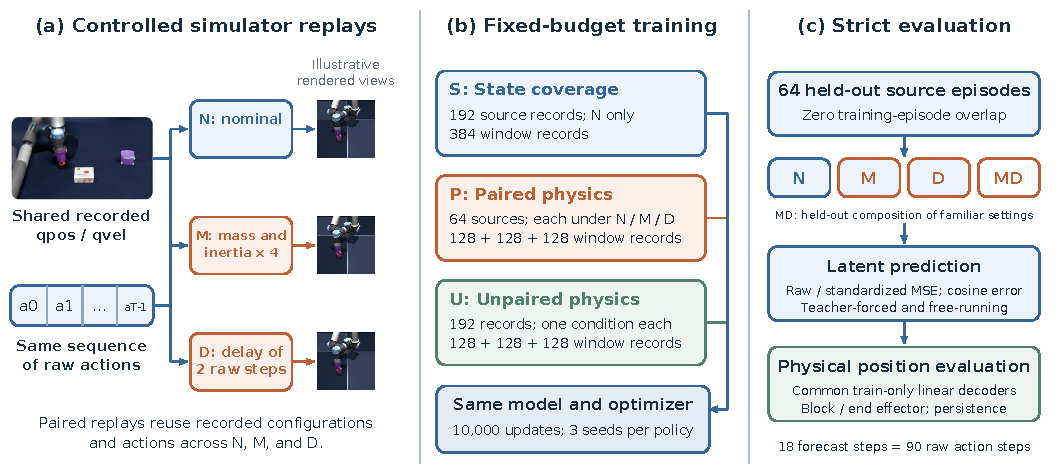
\includegraphics[width=\textwidth]{figures/revised_protocol.pdf}
\caption{Data-collection and evaluation framework. (a) Paired replays reuse recorded configurations and raw actions across nominal (N), mass-and-inertia (M), and delay (D) settings. Robot views illustrate the task and are not a measured comparison of variant trajectories. (b) State, paired, and unpaired policies each use 384 window records, the same model, and 10,000 updates; distinct source counts are given in Table~\ref{tab:data}. (c) Evaluation uses 64 source-episode-disjoint test episodes. MD is a held-out composition of familiar settings. Common physical-state decoders use nominal training calibration only. Closed-loop control is not evaluated for these nine checkpoints.}
\label{fig:protocol}
\end{figure*}

\subsection{Model, Optimization, and Reused Runs}
We use a randomly initialized LeWorldModel with a vision transformer (ViT) image encoder \cite{dosovitskiy2021vit} in the ViT-tiny configuration, a 192-dimensional projected latent, a six-layer action-conditioned predictor, and a 25-dimensional raw-action block encoder. Three latent frames form the predictor history. RGB values are scaled to $[0,1]$ and normalized with channel means $(0.485,0.456,0.406)$ and standard deviations $(0.229,0.224,0.225)$. Training combines prediction error and SIGReg, with no pairing-specific term, no physical-state supervision, and no contact-specific loss weighting. Table~\ref{tab:training} gives the shared settings; MLP denotes a multilayer perceptron \cite{goodfellow2016deeplearning}, and BF16 denotes the bfloat16 numerical format.

There are three trained models per principal policy. State seeds are 0, 1, and 3; paired and unpaired seeds are 0, 1, and 2. The state and paired checkpoints are reused from the completed strict-split study and factor ablation. Their saved arguments agree except for seed, run identifier, and policy-specific data paths. The unpaired runs use the same trainer and settings. We evaluate the final 10,000-update checkpoint in every case; no checkpoint is chosen using test errors. Equal update counts match the training budget, rather than guaranteeing identical wall-clock time. New runs took approximately 32--47 minutes each on NVIDIA A800 GPUs under shared-server conditions.

\begin{table}[t]
\centering
\caption{Shared model and training settings for all principal policies. Models are initialized randomly; only the data policy and random seed vary.}
\label{tab:training}
\footnotesize
\setlength{\tabcolsep}{5pt}
\renewcommand{\arraystretch}{1.12}
\begin{tabular}{p{0.44\columnwidth}p{0.43\columnwidth}}
\toprule
Setting & Value \\
\midrule
Image encoder & ViT-tiny, 12 layers, patch size 14 \\
Image / latent dimensions & $224\times224$ RGB / 192 \\
Predictor & 6 layers, 16 heads, head width 64 \\
Predictor MLP / dropout & 2,048 / 0.1 \\
History / training window & 3 / 10 latent frames \\
Raw actions per latent step & 5 (25 action coordinates) \\
Optimizer / batch size & AdamW / 32 \\
Learning rate / weight decay & $5\times10^{-5}$ / $10^{-3}$ \\
Updates / warmup & 10,000 / 2,000 \\
Schedule / precision & Linear warmup, cosine / BF16 \\
SIGReg weight / projections & 0.09 / 1,024 \\
Gradient-norm clipping & 1.0 \\
Model seeds per main policy & 3 \\
\bottomrule
\end{tabular}
\end{table}


\section{Evaluation and Statistical Analysis}
\subsection{Latent Prediction Metrics}
Let $z_t=e(o_t)\in\mathbb{R}^{d}$, with $d=192$, denote the projected latent. A teacher-forced prediction uses the true three-frame history and the corresponding action blocks. A free-running prediction initializes the history with true frames 0, 1, and 2, and then recursively inserts each prediction into the history. Both evaluations predict frames 3--20. The horizon is therefore $H=18$ latent steps, or 90 raw action steps beyond the last observed frame. All policies use the same test groups and actions.

For test group $g$, raw rollout MSE is
\begin{equation}
 E_g^{\mathrm{raw}}=\frac{1}{Hd}\sum_{h=1}^{H}
 \left\|\hat z_{g,h+2}-z_{g,h+2}\right\|_2^2.
\end{equation}
Teacher-forced MSE uses the same target frames with true histories. Cosine error is $1-\cos(\hat z,z)$, averaged over the same frames. These quantities compare predictions with targets from the \emph{same} trained encoder; no alignment between different models' latent spaces is assumed.

To examine coordinate-scale sensitivity, we additionally compute
\begin{equation}
 E_g^{\mathrm{std}}=\frac{1}{Hd}\sum_{h=1}^{H}\sum_{j=1}^{d}
 \frac{(\hat z_{g,h+2,j}-z_{g,h+2,j})^2}
 {\max(\sigma_j,10^{-6})^2},
\label{eq:standardized}
\end{equation}
where $\sigma_j$ is the population standard deviation of latent coordinate $j$ on the common nominal calibration set described below, calculated separately for each model. This adjustment removes marginal coordinate scale but does not align representations, whiten their covariance, or establish a representation-invariant metric. Raw, standardized, and cosine errors are reported together rather than selecting the metric with the most favorable ranking.

\subsection{Common Train-Only Physical-State Decoders}
\label{sec:decoder}
For every frozen world model, we use the same nominal training groups 0--191 and frames 0--19 as labeled calibration data: 3,840 frame records. Targets are the six coordinates of block and end-effector position in meters. This common calibration set is intentionally independent of each world model's training-source subset; it is an additional, equal evaluation resource, not additional world-model training. It contains no test episodes and no M, D, or MD targets.

A linear ridge decoder maps projected latents to these six coordinates. Hyperparameter selection uses a common split of the 128 calibration source episodes: 102 fitting episodes and 26 validation episodes, with seed 20261030. All starts from an episode stay in the same partition, including the duplicate key. Features and targets are standardized using fitting rows only. For standardized design matrix $X$ and targets $Y$, the fitted coefficient matrix is
\begin{equation}
 W_\alpha=(X^\top X/n+\alpha I)^{-1}X^\top Y/n.
\end{equation}
We choose $\alpha$ from $\{10^{-5},10^{-4},10^{-3},10^{-2},10^{-1},1,10\}$ by the mean validation squared error across standardized target coordinates, then refit on all calibration rows. Decoder parameters and validation scores are retained. No test label participates in fitting, standardization, or hyperparameter selection.

The primary physical endpoint is mean Euclidean block-position error over the same 64 test groups and 18 future frames:
\begin{equation}
 E^{\mathrm{pos}}=\frac{1}{GH}\sum_{g=1}^{G}\sum_{h=1}^{H}
 \left\|D_b(\hat z_{g,h+2})-p^b_{g,h+2}\right\|_2.
\end{equation}
We also evaluate end-effector position. Tables express these errors in centimeters. To separate decoder limitations from recursive prediction, we report decoding from observed future latents, teacher-forced predictions, and free-running predictions. Two persistence references hold either the decoded frame-2 position or the true frame-2 simulator position fixed. The true-state reference has privileged state information and is not an equal-input visual controller.

A linear decoder can fail to recover information present nonlinearly in a representation. Physical errors also combine representation, decoder, and dynamics errors. Consequently, lack of improvement under this protocol is not proof that all physically relevant information is absent. It does test whether the latent ranking translates into improved positions under a fixed, transparent readout procedure.

\subsection{Aggregation and Uncertainty}
\label{sec:stats}
For every checkpoint, each endpoint is first averaged over future frames within a test group and then equally over the 64 test groups. We report the mean of three checkpoint means and their sample standard deviation. Each strict test group corresponds to a different source episode, so group resampling is also episode resampling.

Two percentile bootstrap procedures use 10,000 replicates and seed 20261030. The conditional group-only procedure first averages models within each policy, then resamples the paired test groups. The seed-and-group procedure independently resamples model seeds with replacement within each compared policy, resamples one common set of test-group indices for both policies, and recomputes the difference. Training seed labels are not treated as matched experimental pairs. The main contrast table uses seed-and-group intervals; both interval types are retained in the accompanying numerical results.

Three training seeds provide a limited estimate of training variability. These intervals describe uncertainty conditional on this dataset construction and do not include repeated simulator-pool generation or repeated unpaired assignments. They are unadjusted, descriptive 95\% intervals rather than familywise significance guarantees across all endpoints and conditions. MD raw rollout MSE and MD block-position error are the designated main endpoints of the added comparison; the remaining metrics diagnose the scope of those results. The evaluation and decoder-selection rules were fixed before the new unpaired runs, but the study is not a preregistered experiment.

\section{Results}
\subsection{Raw Latent Error and the Unpaired Baseline}
Table~\ref{tab:latent} reports the held-out MD condition. Paired collection gives raw rollout MSE $1.3623\pm0.0039$, compared with $1.4101\pm0.0092$ for state coverage and $1.4109\pm0.0100$ for unpaired physics coverage. The paired-minus-unpaired difference is $-0.0486$, a 3.45\% reduction, with seed-and-group interval $[-0.0732,-0.0238]$. The paired-minus-state reduction is 3.39\%, with interval $[-0.0729,-0.0238]$. The latter uses three state seeds and therefore replaces the earlier two-state-seed estimate.

The unpaired mixture is close to the state baseline: difference $+0.0008$, interval $[-0.0254,0.0291]$. This result does not show that physics variation in general is ineffective; it shows no clear raw-rollout benefit for this particular independent assignment and budget. Paired raw-rollout advantages also appear on the three other test conditions (Table~\ref{tab:variants}). These conditions reuse the same test episodes and should not be interpreted as four independent replications.

\begin{table*}[t]
\centering
\caption{Latent metrics on held-out MD for the strict source-episode split. Entries are mean $\pm$ sample standard deviation over three training seeds. Errors average 64 test groups and 18 future frames; lower is better. Standardization uses model-specific coordinate deviations from the common nominal training calibration set.}
\label{tab:latent}
\small
\setlength{\tabcolsep}{5pt}
\renewcommand{\arraystretch}{1.12}
\begin{tabular}{lrrr}
\toprule
Metric & State (S) & Paired (P) & Unpaired (U) \\
\midrule
Teacher-forced MSE & $1.2006\pm0.0145$ & $1.1903\pm0.0145$ & $1.2058\pm0.0145$ \\
Teacher-forced cosine error & $0.8221\pm0.0037$ & $0.8611\pm0.0042$ & $0.8222\pm0.0062$ \\
Raw rollout MSE & $1.4101\pm0.0092$ & $1.3623\pm0.0039$ & $1.4109\pm0.0100$ \\
Standardized rollout MSE & $1.4103\pm0.0125$ & $1.4226\pm0.0175$ & $1.4497\pm0.0112$ \\
Rollout cosine error & $0.9101\pm0.0100$ & $0.9353\pm0.0131$ & $0.9100\pm0.0040$ \\
\bottomrule
\end{tabular}
\end{table*}

\begin{table*}[t]
\centering
\caption{Policy differences on held-out MD with 95\% percentile intervals resampling training seeds independently within policies and test groups jointly (10,000 replicates). Negative values favor the first policy in the contrast. Intervals are descriptive and unadjusted across endpoints.}
\label{tab:contrasts}
\footnotesize
\setlength{\tabcolsep}{5pt}
\renewcommand{\arraystretch}{1.12}
\begin{tabular}{lccc}
\toprule
Endpoint & P $-$ S & P $-$ U & U $-$ S \\
\midrule
Raw rollout MSE & $-0.0478$ $[-0.0729,-0.0238]$ & $-0.0486$ $[-0.0732,-0.0238]$ & $+0.0008$ $[-0.0254,+0.0291]$ \\
Standardized rollout MSE & $+0.0123$ $[-0.0178,+0.0429]$ & $-0.0271$ $[-0.0553,+0.0054]$ & $+0.0394$ $[+0.0116,+0.0693]$ \\
Rollout cosine error & $+0.0252$ $[+0.0070,+0.0461]$ & $+0.0253$ $[+0.0095,+0.0450]$ & $-0.0001$ $[-0.0162,+0.0165]$ \\
Block position (cm) & $+1.04$ $[-0.51,+2.52]$ & $+0.62$ $[-1.33,+2.46]$ & $+0.41$ $[-1.23,+2.06]$ \\
End-effector position (cm) & $+0.86$ $[-0.74,+2.42]$ & $+0.50$ $[-1.47,+2.41]$ & $+0.36$ $[-1.26,+1.95]$ \\
\bottomrule
\end{tabular}
\end{table*}

\begin{table*}[t]
\centering
\caption{Raw rollout MSE across the four strict test conditions (same 64 episodes). Each policy has three training seeds. The final column gives the paired-minus-unpaired difference with a seed-and-group 95\% interval. N, M, and D are seen training conditions for physics-diverse policies; MD is a held-out composition.}
\label{tab:variants}
\footnotesize
\setlength{\tabcolsep}{5pt}
\renewcommand{\arraystretch}{1.12}
\begin{tabular}{lrrrc}
\toprule
Condition & State (S) & Paired (P) & Unpaired (U) & P $-$ U \\
\midrule
N & $1.3957\pm0.0054$ & $1.3608\pm0.0108$ & $1.3938\pm0.0143$ & $-0.0330$ $[-0.0605,-0.0058]$ \\
M & $1.3966\pm0.0090$ & $1.3627\pm0.0060$ & $1.3945\pm0.0183$ & $-0.0318$ $[-0.0595,-0.0036]$ \\
D & $1.4071\pm0.0078$ & $1.3679\pm0.0047$ & $1.4096\pm0.0135$ & $-0.0417$ $[-0.0683,-0.0157]$ \\
MD & $1.4101\pm0.0092$ & $1.3623\pm0.0039$ & $1.4109\pm0.0100$ & $-0.0486$ $[-0.0732,-0.0238]$ \\
\bottomrule
\end{tabular}
\end{table*}


\subsection{The Ranking Depends on the Latent Metric}
The raw-rollout ranking does not hold across metrics. After coordinate standardization, paired MSE is 1.4226 versus 1.4103 for state coverage. Their difference, $+0.0123$, has seed-and-group interval $[-0.0178,0.0429]$. The standardized paired-minus-unpaired interval also includes zero. Rollout cosine error is higher for paired collection than for either alternative; the paired-minus-state difference is $+0.0252$, with interval $[0.0070,0.0461]$. Teacher-forced MSE differences are smaller than the raw-rollout differences and do not establish a broad improvement across latent metrics.

Figure~\ref{fig:contrasts} illustrates this disagreement. It makes coordinate scale a plausible contributor to the raw-MSE ranking, but does not identify scale as its sole cause: coordinate standardization changes the weighting of dimensions and cannot make independently learned representations equivalent. The supported result is a reduction in raw latent rollout error under the specified collection policy, not a representation-independent improvement in dynamics.

\begin{figure*}[t]
\centering
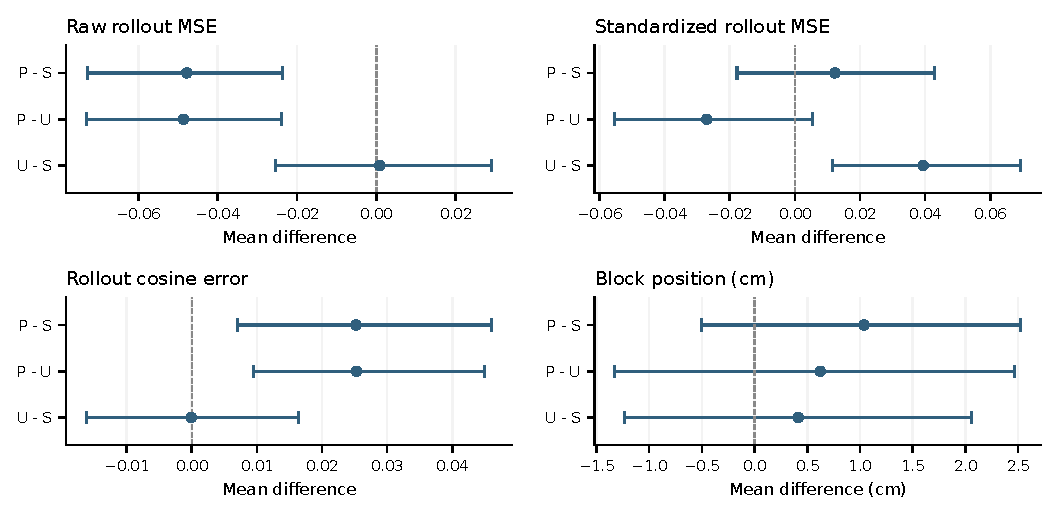
\includegraphics[width=\textwidth]{figures/metric_contrasts.pdf}
\caption{Policy differences on held-out MD. Points are mean differences; intervals resample both training seeds and common test episodes. S, P, and U denote state, paired, and unpaired policies. Negative values favor the first policy in each contrast. The raw-MSE advantage does not persist uniformly across coordinate-standardized MSE, cosine error, and decoded block-position error. Panel scales and units differ.}
\label{fig:contrasts}
\end{figure*}

\subsection{Decoded Physical Prediction}
Table~\ref{tab:physical} reports physical errors for all decoding modes. Free-running block-position errors are $14.87\pm0.36$ cm for state coverage, $15.91\pm0.87$ cm for paired coverage, and $15.28\pm1.27$ cm for unpaired coverage. Paired minus state is $+1.04$ cm, with seed-and-group interval $[-0.51,2.52]$ cm. The mean is worse, but the interval does not establish a reliable deterioration across training seeds. The comparisons with unpaired coverage similarly do not establish a physical improvement. End-effector errors lead to the same qualitative conclusion.

Observed-future-latent block decoding already incurs approximately 11.5--11.8 cm error. This exposes a substantial readout limitation before dynamics predictions are introduced. The privileged true-state persistence reference has block error 13.46 cm, below the mean free-running error of all three policies, although it receives true initial position rather than images. These references qualify what can be inferred from the physical evaluation; they are not evidence of successful control. Figure~\ref{fig:horizon} reports errors by forecast step without choosing a favorable horizon.

\begin{table*}[t]
\centering
\caption{Physical position errors on strict held-out MD, in centimeters (mean $\pm$ sample seed standard deviation; three models per policy). All entries use 64 test groups and the same 18 future frames. Observed-latent decoding measures readout error without dynamics prediction. True-state persistence has privileged initial simulator position and is only a reference.}
\label{tab:physical}
\footnotesize
\setlength{\tabcolsep}{5pt}
\renewcommand{\arraystretch}{1.12}
\begin{tabular}{lrrrrrr}
\toprule
Prediction / reference & \multicolumn{3}{c}{Block position} & \multicolumn{3}{c}{End-effector position} \\ & S & P & U & S & P & U \\
\midrule
Observed future latent & $11.51\pm0.30$ & $11.78\pm0.52$ & $11.58\pm0.08$ & $10.85\pm0.36$ & $11.06\pm0.50$ & $10.94\pm0.17$ \\
Teacher-forced prediction & $11.44\pm0.19$ & $12.23\pm0.36$ & $11.57\pm0.08$ & $10.86\pm0.31$ & $11.54\pm0.36$ & $11.03\pm0.21$ \\
Free-running prediction & $14.87\pm0.36$ & $15.91\pm0.87$ & $15.28\pm1.27$ & $14.41\pm0.32$ & $15.27\pm1.01$ & $14.77\pm1.26$ \\
Decoded-state persistence & $16.66\pm0.39$ & $17.29\pm0.33$ & $17.32\pm0.50$ & $16.89\pm0.58$ & $17.38\pm0.41$ & $17.45\pm0.32$ \\
True-state persistence & $13.46\pm0.00$ & $13.46\pm0.00$ & $13.46\pm0.00$ & $15.25\pm0.00$ & $15.25\pm0.00$ & $15.25\pm0.00$ \\
\bottomrule
\end{tabular}
\end{table*}

\begin{figure*}[t]
\centering
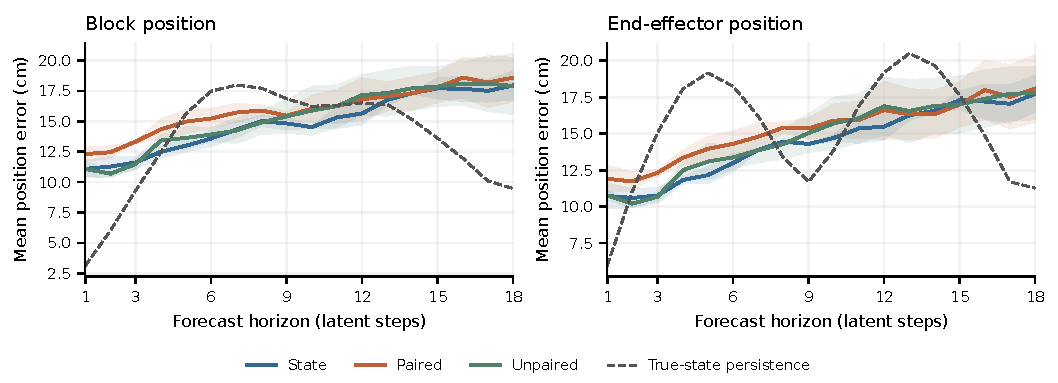
\includegraphics[width=\textwidth]{figures/physical_horizon.pdf}
\caption{Decoded free-running position error versus forecast horizon on MD, averaged over three seeds and 64 test episodes. Shading denotes one standard deviation across checkpoint-level curves, not a confidence interval. The dashed reference holds the true frame-2 position fixed and uses privileged simulator state. Each latent step spans five raw actions.}
\label{fig:horizon}
\end{figure*}

\subsection{Single-Factor Results}
An existing strict-split ablation uses nominal-plus-M or nominal-plus-D data from groups 0--95, with two windows per condition and group. Each factor policy has 384 window records and two model seeds; it is compared with the same three-state-seed baseline. Table~\ref{tab:factor} reports MD raw rollout results and seed-and-group intervals recomputed from the saved group-level errors.

Mass-only coverage reduces raw rollout MSE by 8.1\%, whereas delay-only coverage does not clearly change it. These results are conditional on different source reuse: a factor policy covers 96 source groups, while the paired three-condition policy covers 64. The larger mass-only effect therefore does not show that delay is intrinsically harmful. Moreover, the factor checkpoints were not included in the new standardized-latent and physical-decoder evaluation; their raw-MSE advantages must not be interpreted as demonstrated physical gains.

\begin{table*}[t]
\centering
\caption{Exploratory strict-split single-factor ablation on MD. Factor policies use 96 source groups and 384 window records each, with two training seeds. The common state reference has three seeds and raw rollout MSE $1.4101\pm0.0092$. Differences are factor minus state, with seed-and-group 95\% intervals recomputed from saved per-group outputs. Standardized and physical-decoder results were not measured for these factor checkpoints.}
\label{tab:factor}
\footnotesize
\setlength{\tabcolsep}{5pt}
\renewcommand{\arraystretch}{1.12}
\begin{tabular}{lrrrc}
\toprule
Factor policy & Source groups & Seeds & Raw rollout MSE & Difference [95\% interval] \\
\midrule
Nominal + M & 96 & 2 & $1.2955\pm0.0303$ & $-0.1146$ $[-0.1522,-0.0750]$ \\
Nominal + D & 96 & 2 & $1.4155\pm0.0069$ & $+0.0054$ $[-0.0223,+0.0323]$ \\
\bottomrule
\end{tabular}
\end{table*}


\Needspace{6\baselineskip}
\section{Discussion and Limitations}
\subsection{What the Added Comparison Establishes}
The unpaired mixture addresses a specific missing comparator. Merely including N, M, and D at equal proportions does not reproduce the paired policy's raw-MSE result in this experiment. However, the policies differ in source-state and action reuse, and the training objective never consumes pair identities. Repetition across conditions could alter the learned representation, the effective weighting of source trajectories, or dynamics learning. The experiment does not distinguish these explanations. An experiment that isolates correspondence at fixed unique-state and action coverage would require a different construction.

The disagreement between raw, standardized, angular, and physical metrics is itself a useful empirical observation. A data-collection decision justified solely by raw latent MSE could have a different ranking when the downstream quantity is a physical position. We therefore recommend interpreting the present results as a measurement-sensitive comparison of collection policies, rather than a general rule that mechanism coverage dominates state coverage.

\subsection{Scope of Generalization and Downstream Evidence}
The study uses one simulator task, one visual configuration, one model family, one strict source split, and one fixed unpaired assignment. Test source episodes are new, but the mass values and delay values are familiar. No interpolation or extrapolation to new masses, visual-domain transfer, real-robot evaluation, or longer-budget replication is established. The 10,000-update training regime is also much narrower than a full assessment of LeWorldModel's achievable control performance.

The principal nine checkpoints have not been evaluated for successful closed-loop control in the added experiment. Earlier inverse-dynamics control results belong to a different development dataset and are reported separately in Appendix~\ref{app:development}. They cannot be presented as control results for the strict-split models. A failed low-budget controller would in any case provide little resolution for ranking otherwise similar representations.

\subsection{Data and Measurement Limitations}
Matching window-record and update budgets does not match distinct dynamical sources exactly. The duplicate source key and differing rendered pixels are reported rather than silently corrected after training. The audit verifies recorded configurations and action arrays, but not every hidden simulator variable. The unpaired subsets also have finite-sample differences in state and action distributions. Repeated data assignments and fully specified simulator-state restoration would be needed to assess robustness to these choices.

The linear-decoder evaluation controls calibration data and selection procedures across models but is not invariant to nonlinear changes of representation. Conversely, standardized latent MSE only addresses marginal coordinate scales, not rotations or broader representation geometry. Neither metric alone supplies a definitive measure of physical understanding. With three seeds per main policy and two per factor policy, uncertainty about training variability remains substantial.

\section{Conclusion}
Under a fixed window-record and update budget, paired physics collection produces lower raw latent rollout MSE than either nominal state coverage or an unpaired physics mixture on OGBench Cube. The added unpaired comparison shows that the observed raw-MSE result is not reproduced by matching physical-condition proportions alone. It does not isolate pairing from source reuse or establish causal mechanism identification.

The benefit is limited by the evaluation metric. It does not persist over the state baseline after coordinate standardization, cosine error is worse, and a common train-only linear-decoder protocol does not establish improved physical position prediction. The appropriate conclusion is therefore that collection policy changes latent prediction measurements in this setting, while its physical and control benefits remain unverified. Reporting multiple metrics, source-level data audits, and training-seed uncertainty is necessary to make that distinction visible.

\appendices
\section{Development Experiments and Their Evidence Scope}
\label{app:development}
The earlier experiments below explain the development of the comparison and retain negative findings. They are not pooled with the principal strict-split results.

\subsection{Temporal Sampling}
A separate 20,000-update experiment compares 2,000 training windows from 200 episodes using uniform, high-contact, low-contact, or balanced high/low-contact sampling. High and low contact correspond to the upper and lower quartiles of contact occupancy in candidate windows. The probe episodes are shared across policies and disjoint from their training episodes. Table~\ref{tab:sampling} reports the saved checkpoint-level summaries: contact MSE is teacher-forced latent MSE on contact targets; p95 is its 95th percentile; probes are mean Pearson correlations for decoded state variables. These probes use the earlier experiment's fitting protocol and are not the common ridge-decoder evaluation of Section~\ref{sec:decoder}. The comparison shows that oversampling contact did not minimize its raw latent error, without establishing a general event-sampling rule.
\begin{table*}[t]
\centering
\caption{Earlier temporal-sampling diagnostic: 2,000 windows from 200 training episodes, 20,000 updates, and shared disjoint probe episodes. Values are seed means $\pm$ sample standard deviations. Contact MSE and its p95 are teacher-forced latent errors; probes are mean Pearson correlations. Probe fitting differs from the principal physical evaluation.}
\label{tab:sampling}
\footnotesize
\setlength{\tabcolsep}{5pt}
\renewcommand{\arraystretch}{1.12}
\begin{tabular}{lrrrrr}
\toprule
Sampling policy & Seeds & Contact MSE & Contact p95 & Block probe & Gripper probe \\
\midrule
Uniform & 3 & $1.078\pm0.012$ & $1.460\pm0.017$ & $0.790\pm0.003$ & $0.722\pm0.017$ \\
High contact & 3 & $1.158\pm0.023$ & $1.554\pm0.030$ & $0.762\pm0.002$ & $0.605\pm0.020$ \\
Low contact & 2 & $1.224\pm0.008$ & $1.619\pm0.016$ & $0.756\pm0.019$ & $0.672\pm0.005$ \\
Balanced tails & 2 & $1.091\pm0.000$ & $1.494\pm0.015$ & $0.797\pm0.008$ & $0.710\pm0.027$ \\
\bottomrule
\end{tabular}
\end{table*}


\subsection{Budget Scan on the Earlier Group Split}
Table~\ref{tab:scaling} reports 96, 192, and 384-window comparisons from the earlier dataset, with 10,000 updates at each budget. Its training groups come from 132 source episodes and its test groups from 56 source episodes; 32 episodes appear in both pools. Group identifiers are held out, but source episodes are not. Its group-bootstrap intervals also do not account for possible dependence between test groups from the same source episode. These values are therefore exploratory and are not independent confirmation of the strict-split result.

The relative paired-minus-state difference changes sign across the tested budgets, but absolute errors also change substantially and nonmonotonically in favorability. Fixed update counts imply different numbers of passes over the data. The three points do not establish a universal coverage threshold or a causal scaling law. In particular, the 384-window values 1.3838 and 1.3361 in this table must not be substituted for the principal strict-split values 1.4101 and 1.3623.
\begin{table*}[t]
\centering
\caption{Earlier budget scan on a group-disjoint but source-episode-overlapping dataset. Each run uses 10,000 updates. Values are raw rollout MSE on MD; intervals average model seeds before resampling groups and do not adjust for shared source episodes. These exploratory results are not pooled with the strict-split study.}
\label{tab:scaling}
\footnotesize
\setlength{\tabcolsep}{5pt}
\renewcommand{\arraystretch}{1.12}
\begin{tabular}{rrr rc}
\toprule
Windows & S/P seeds & State (S) & Paired (P) & P $-$ S [group-only 95\% interval] \\
\midrule
96 & 2/2 & $1.0946\pm0.0565$ & $1.2122\pm0.0511$ & $+0.1176$ $[+0.0982,+0.1374]$ \\
192 & 2/2 & $1.2645\pm0.0271$ & $1.2871\pm0.0327$ & $+0.0226$ $[-0.0055,+0.0545]$ \\
384 & 3/4 & $1.3838\pm0.0163$ & $1.3361\pm0.0216$ & $-0.0477$ $[-0.0778,-0.0181]$ \\
\bottomrule
\end{tabular}
\end{table*}


\subsection{Earlier Action Decoding and Direct Control}
On that earlier dataset, inverse-dynamics models fitted to two state and three paired checkpoints obtain normalized action MSE $0.9764\pm0.0273$ and $1.0454\pm0.0113$, respectively; mean action correlations are $0.352\pm0.019$ and $0.324\pm0.009$. Direct inverse-dynamics Cube control yields 0 successes in 20 evaluation episodes for each of those five checkpoints. These were direct inverse-dynamics tests, not evidence of improved model-predictive control or results for the nine principal checkpoints. They document a lack of demonstrated downstream success in development; the source-episode overlap and separate checkpoint set limit their evidential role.

\section{Reproducibility Details}
\label{app:repro}
The experiment package includes the fixed data-assignment audit, model/optimization settings, evaluation and aggregation scripts, per-model physical metrics, and summary statistics. Numerical tables in this manuscript are generated from saved JSON reports. Strict-split physical evaluation independently recomputes latent metrics; the largest per-group discrepancy from the original evaluator across the nine checkpoints and four conditions is approximately $1.1\times10^{-6}$, below the specified $2\times10^{-4}$ tolerance.

The recorded software environment is PyTorch 2.5.1 with CUDA 12.4, torchvision 0.20.1, NumPy 2.2.6, SciPy 1.15.3, h5py 3.16.0, MuJoCo 3.8.0, OGBench 1.2.1, and Transformers 5.6.2. The underlying model-code revision is \code{ca231f9f9d9a}; the data-study revision preceding the added scripts is \code{0fc2b7382b22}. The source and protocol hashes for the added runs are retained with the experiment records. These identifiers describe the recorded software environment; the supplementary code and numerical data are publicly available as specified below.

\section*{Data and Code Availability}
The supplementary code and numerical data are publicly available at \url{https://github.com/ArmstrongAviation/state-physics-coverage}. The repository includes experiment scripts, evaluation reports, non-image simulator state/action arrays, fitted ridge-decoder parameters, training metadata, and CPU-only numerical reproduction tools. Full RGB replay trajectories, the source expert HDF5 dataset, and world-model checkpoint weights are not included. Instructions, software requirements, and limitations are documented in the repository README.

\section*{Acknowledgment}
OpenAI Codex \cite{openai2026codex} assisted with drafting and restructuring the abstract, main text, appendices, and captions, and with developing the additional evaluation, aggregation, and manuscript-generation scripts. Reported experimental values are computed from saved training and evaluation outputs.

\FloatBarrier
\bibliographystyle{IEEEtran}
\bibliography{references}
\raggedbottom
\begin{IEEEbiography}[{
\includegraphics[width=1in,height=1.25in,keepaspectratio]{authors_image/yanfei_liu.jpeg}}]{Yanfei Liu}
received the M.S. degree in computer application technology from Henan Polytechnic University, Jiaozuo, China, in 2008. She is currently an Associate Professor and the Program Director of the Artificial Intelligence Technology Application Program with the School of Information Engineering, Zhongshan Polytechnic, Zhongshan, China. She has presided over more than 20 research and education projects, including provincial key projects on citrus harvesting intelligent robots and a Zhongshan City key scientific research project entitled ``Research and Application of Dualarm Collaborative Intelligent Picking Robot for Pitaya Based on Deep Reinforcement Learning.'' Her research interests include agricultural robotics and dexterous manipulation, data-centric imitation learning, intelligent perception, and artificial intelligence technology education.
\end{IEEEbiography}

\begin{IEEEbiography}[{
\includegraphics[width=1in,height=1.25in,keepaspectratio]{authors_image/liangzhong_lin.jpeg}}]{Liangzhong Lin}
received the Ph.D. degree in theoretical condensed matter physics from the Institute of Semiconductors, Chinese Academy of Sciences, Beijing, China, in 2014. He is currently a teacher of the Artificial Intelligence program at Zhongshan Polytechnic, Zhongshan, China. His research interests include the fundamental physics of semiconductors in mesoscopic systems, such as spin manipulation in two-dimensional electron gas (2DEG) and spin field effects in quasi-one-dimensional electron gas (Q1DEG), as well as semiconductor optoelectronics, intelligent LED control, AI technology applications, and data-centric intelligent systems.
\end{IEEEbiography}

\begin{IEEEbiography}[{
\includegraphics[width=1in,height=1.25in,keepaspectratio]{authors_image/zhiying_cao.png}}]{Zhiying Cao}
received the Ph.D. degree in signal and information processing from the University of Chinese Academy of Sciences. He used to be a Principal Algorithm Engineer and the Head of the Perception Model Development Section with the Automotive New Technology Research Institute, BYD Auto Industry Company Limited, Shenzhen, China. His research interests include data-centric autonomous driving perception, dataset quality governance, deep learning model compression, and computer vision.
\end{IEEEbiography}

\begin{IEEEbiography}[{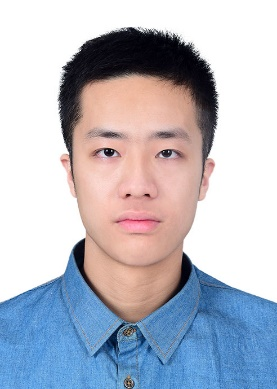
\includegraphics[width=1in,height=1.25in,keepaspectratio]{authors_image/chengliang_li.jpeg}}]{Chengliang Li}
is currently pursuing the B.S. degree in computer science and technology at Beijing Normal-Hong Kong Baptist University (BNBU), Zhuhai, China. He is an undergraduate student and expects to graduate in 2027. His research interests include robotics and embodied intelligence.
\end{IEEEbiography}

\begin{IEEEbiography}[{
\includegraphics[width=1in,height=1.25in,keepaspectratio]{authors_image/weichang_li.jpeg}}]{Weichang Li}
received the B.S. degree and the M.Phil. degree in mechanical engineering from Guangdong University of Technology, Guangzhou, China, in 2019 and 2021, respectively. He is currently pursuing the Ph.D. degree in control engineering with the School of Automation Science and Engineering, South China University of Technology, Guangzhou, China. His research interests include the application of advanced control theory in real-world robotics.
\end{IEEEbiography}

\EOD
\end{document}
